Die Aufgabe der \emph{automatischen Klassifizierung} ist es, eine deterministische Funktion (oder ein Klassifikator beziehungsweise ein Klassifikationsverfahren) $f(x)$ anhand von \emph{Trainingsdaten} zu finden, die gewissen Daten $x \in \mathcal{X}$ eine (zu den Daten charakteristische) Klasse $y \in \mathcal{Y}$ zuweist. Verfahren dieser Art bezeichnen wir als \emph{(Lern-)Maschine} (\cite{b-tut-1998}). Die \emph{Support-Vector-Machine} (SVM) ist eine spezielle Lern-Maschine, die gewisse \glqq gute\grqq{} Eigenschaften besitzt, siehe hierzu \cite{b-tut-1998}. \\

Im folgenden Unterkapitel werden wir ein für uns geeignetes mathematisches Modell für die automatische Klassifizierung formulieren. Die SV-Machine behandeln wir im nächsten Unterkapitel.

\section{Automatische Klassifizierung}
Für die \emph{Textklassifizierung}, die wir später noch einführen werden, sind drei Typen von Klassifikatoren wesentlich.

\begin{definition}[Binär-Klassifikator]
	Sei $L=\{-1,1\}$ die Menge aller Klassen. Unter einem \emph{Binär-Klassifikator} verstehen wir eine Funktion $h:\mathbb{R}^n \rightarrow L$, die einem Datenvektor eine Klasse zuweist.
\end{definition}

\begin{definition}[Multi-Label-Klassifikator] \label{def:mlk}
	Sei $L=\{0 , 1 , 2 , ... , k\}$ die Menge aller Klassen. Unter einem \emph{Multi-Label-Klassifikator} (MLK) verstehen wir eine Funktion $h:\mathbb{R}^n \rightarrow  \mathcal{P}(L)$, die einen Datenvektor auf eine Menge Klassen zuweist. Die Menge $\mathcal{P}(L)$ bezeichnet die Potenzmenge von $L$.
\end{definition}

\begin{definition}[Multi-Klassen-Klassifikator]
	Sei $L=\{1 , 2 , ... , k\}$ die Menge aller Klassen. Unter einem \emph{Multi-Klassen-Klassifikator} (MKK) verstehen wir eine Funktion $h:\mathbb{R}^n \rightarrow  L$, die einen Datenvektor genau eine Klasse zuweist. 
\end{definition}

\begin{algorithm}[bhtp]
\KwIn{$x \in \mathbb{R}^n$}
\KwOut{$A \subset L$}
\KwData{Binärklassifikatoren $h_1,...,h_l$ bezüglich der einzelnen Klassen $1,...,l$}
$A \gets \{ \; \}$ \;
\ForEach{$i \in L$}{
	\If{$h_i(x) = 1$}{
		$A \gets A \cup \{i\}$
	}
}
\caption{Ein aus Binär-Klassifikatoren konstruierter MLK.}
\label{alg:mlk}
\end{algorithm}

Der Multi-Label-Klassifikator ist bei der Textklassifizierung nützlich, da die Textdokumente durchaus mehreren Themen zugeordnet werden können. Wie in Algorithmus \ref{alg:mlk} dargestellt lässt sich jeder MLK durch Binärklassifikatoren darstellen. Wir werden in Experiment C (Abschnitt \ref{sec:exp-c}) jedoch auf einen MKK zurückgreifen. Auch der MKK kann in vielen Fällen - und so auch bei der SVM - mit der \emph{one-vs-rest} Strategie (siehe \cite{hsu-comp-02}) über Binärklassifikatoren gewonnen werden. Aus diesem Grund wollen wir uns zunächst auf die Binärklassifikatoren beschränken. Im Abschnitt \nameref{sec:ovr} (Unterkapitel \ref{sec:ovr}) werden wir dann auf die Konstruktion eines MKKs genauer eingehen. Wir können also von folgendem Setting ausgehen: \\

Seien $(x^1,y^1),(x^2,y^2),...,(x^l,y^l)$ Trainingsdaten, wobei $x^i \in \mathbb{R}^n$  und $y^i \in \{-1,1\}$ die entsprechende Klasse für $1 \leq i \leq l$ sind. Wir werden wir immer fordern, dass $n\geq 2,\ x^i \neq 0$, sowie $y^i \neq y^j$ für alle  $1 \leq i \leq l$ und mindestens ein $j,\  1 \leq j \leq l$ gelten. \\


Eine Qualitätsgröße für einen Klassifikators liefert uns das \emph{empirische Risiko}:
\begin{definition}[Empirisches Risiko]
	Sei $h: \mathbb{R}^n \rightarrow \{-1,1\}$. Dann ist das empirische Risiko definiert durch
	\begin{equation}
	R_{emp}(h) := \frac{1}{l} \cdot \sum_{i=1}^{l}{\mathds{1}_{\{ h \neq y^i \}}(x^i)},
	\end{equation}
	wobei mit $\mathds{1}_{A}$ die \emph{Indikatorfunktion} gemeint ist und die Menge $A=\{ h \neq y^i \}=\{ x \in \mathbb{R}^n \ | \ h(x) \neq y^i \}$ gesetzt wurde. 
\end{definition}

Das empirische Risiko schätzt also den zu erwartenden Fehler bei Anwendung des Klassifikationsverfahrens. Wir werden später illustrieren, dass das empirische Risiko alleine nicht unbedingt ein vertrauensvolle Größe für die Abschätzung der \emph{Generalisierungsfähigkeit} eines Klassifikators ist. Nach \cite{sb-umlfta} lässt sich eine höhere Generalisierungsfähigkeit hingegen durch bestimmte einschränkende Bedingungen an die zu betrachtende Funktionsklasse $\mathbb{H} \subset \{ \, h \, \mid  \, h: \mathbb{R}^n \rightarrow \{-1 ,\ 1\} \, \}$ bewerkstelligen. Hat man eine Funktionsklasse $\mathbb{H}$ gegeben, so kann eine Lern-Maschine beispielsweise den Klassifikator aus $\mathbb{H}$ auswählen, der das empirische Risiko bezüglich der gegebenen Trainingsdaten minimiert.

\begin{definition}[Empirische Risikominimierung]
	\label{definition-erm}
	Sei $\mathbb{H} \subset \{ \, h \, \mid  \, h: \mathbb{R}^n \rightarrow \{-1 ,\ 1\} \, \}$.
	Wir bezeichnen das Problem
	\begin{equation}
	\label{equ-erm}
	h^*(x) := \argmin_{h \in \mathbb{H}} R_{emp}(h)
	\end{equation}
	als \emph{empirische Risikominimierung} bezüglich $\mathbb{H}$. Hat  (\ref{equ-erm}) eine Lösung $h^*$, so bezeichnen wir mit $h^*$ einen optimalen Klassifikator (bezüglich $\mathbb{H}$).
\end{definition}

Die empirische Risikominimierung kann uns also eine Anleitung für die Konstruktion einer Lernmaschine liefern. 

\section{Lineare Klassifikatoren}
Eine einfache Funktionsklasse, die bei bestimmten Problemen durchaus Anwendung findet, ist die Klasse der \emph{linearen Klassifikatoren} (Definition \ref{def-lin-klass}). Diese doch starke Einschränkung wirkt sich im Allgemeinen sicherlich nicht minimierend auf das empirische Risiko aus. Auf der anderen Seite kann die Einschränkung jedoch für eine höhere Generalisierungsfähigkeit hilfreich sein, siehe hierzu \cite{sb-umlfta}. Wir wollen die \glqq linearen Klassifikatoren\grqq{} nun mathematisch formulieren. Hierfür werden wir zunächst ein paar Definitionen einführen.

\begin{definition}[Hyperebene]
	\label{def-hyperebene}
	Seien $(w,b) \in \mathbb{R}^n \times \mathbb{R}$. Wir nennen die Menge
	\begin{equation}
		\label{hyperebene}
		E_{(w,b)}=\{ x \in \mathbb{R}^n \mid w^tx + b = 0 \}
	\end{equation}
	\emph{Hyperebene} im Raum $\mathbb{R}^n$ bezüglich $(w,b)$. Oft werden wir auch von der Hyperebene $(w,b)$ sprechen, wobei immer die durch $(w,b)$ induzierte Menge (\ref{hyperebene}) gemeint ist.
\end{definition}

\begin{definition}[Abstand zur Hyperebene]
	Seien $x \in \mathbb{R}^n, \ (w,b) \in \mathbb{R}^n \times \mathbb{R}$. Dann ist 
	der Abstand von $x$ zur Hyperebene $E_{(w,b)}$ durch
	\begin{equation}
		d(E_{(w,b)},x) := \inf_{y \in E_{(w,b)}} ||y-x||
	\end{equation}
	definiert.
\end{definition}

\begin{lemma}
	\label{lemma-abstand-norm}
	Seien $x \in \mathbb{R}^n, \ (w,b) \in \mathbb{R}^n \times \mathbb{R},\ ||w|| = 1$.
	Dann ist der \emph{Abstand} $d(E_{(w,b)},x)$ von $x$ zur Hyperebene $E_{(w,b)}$ durch $| \langle w,x \rangle +b |$ gegeben.
\end{lemma}
\begin{proof}
	Siehe hierzu beispielsweise den Beweis von Behauptung 15.1. in \cite{sb-umlfta}.
\end{proof}

\begin{lemma}
	\label{lemma-abst-hyp-allg}
	Seien $x \in \mathbb{R}^n, \ (w,b) \in \mathbb{R}^n \times \mathbb{R}$. 
	Dann ist der Abstand $d(E_{(w,b)},x)$ von $x$ zur Hyperebene $E_{(w,b)}$ durch
	$\frac{1}{||w||}|\langle w,x \rangle + b|$
	gegeben.
\end{lemma}
\begin{proof}
	Setze $\tilde{w} := \frac{w}{||w||}$ und $\tilde{b} := \frac{b}{||w||}$. Dann ist der Abstand zwischen $x$ und der Hyperebene $(\tilde{w},\hat{b})$ nach dem vorherigen Lemma
 	$\langle \tilde{w},x \rangle + \tilde{b} = \frac{1}{||w||}|\langle w,x \rangle + b|$. 
 	Da die Beziehung $E_{(w,b)}=E_{(\tilde{w},\tilde{b})}$ gilt, ist das Lemma bewiesen. 
\end{proof}

\begin{definition}[Lineare Separierbarkeit]
	\label{def-lin-sep}
	Wir sagen, die Vektoren $(x^1,y^1),...,(x^l,y^l)$ mit $x^i \in \mathbb{R}^n$  und $y^i \in \{-1,1\} ,\ 1 \leq i \leq l$ sind genau dann \emph{linear separierbar}, wenn eine Hyperebene $(w,b) \in \mathbb{R}^{n+1}$ existiert, sodass 
	\begin{equation}
		\label{equ-lin-sep}
		y^k(w^tx^k+b) > 0, \ \text{für alle} \ 1 \leq k \leq l
	\end{equation}
	gilt. Weiter sagen wir, $(w,b)$ separiert die Vektoren $(x^1,y^1),(x^2,y^2),...,(x^l,y^l)$ genau dann, wenn (\ref{equ-lin-sep}) gilt. Wir werden Separierbarkeit und lineare Separierbarkeit als Synonyme verwenden. 
\end{definition}

\begin{bemerkung}
	Die Bedingung (\ref{equ-lin-sep}) impliziert, dass der Abstand $d(E_{(w,b)},x^k)$ aller Datenvektoren 
	$x^k, \ \text{mit} \ 1 \leq k \leq l$ zur Hyperebene $E_{(w,b)}$ positiv $(> 0)$ sein muss. Weiter legt  (\ref{equ-lin-sep}) genau fest, in welchen der durch die Hyperebene induzierten Halbräumen die Vektoren liegen müssen.
\end{bemerkung}

Solange nicht anders erwähnt, setzen wir im Folgenden die lineare Separierbarkeit der Vektoren $(x^1,y^1),...,(x^l,y^l)$ immer voraus. 

\begin{definition}[Linearer Klassifikator]
	\label{def-lin-klass}
	Wir definieren mit
	\begin{equation}
	h_{(w,b)}(x) := \sign(w^t  x + b)
	\end{equation} 
	einen durch die Hyperebene $(w,b) \in \mathbb{R}^n \times \mathbb{R}$ induzierten \emph{linearen Klassifikator}.
\end{definition} 

Der lineare Klassifikator ist offenbar nur auf der Menge $\mathbb{R}^n \setminus E_{(w,b)}$ sinnvoll definiert. Für Datenvektoren innerhalb der Ebene kann in diesem Setting keine sinnvolle Entscheidung bezüglich der Klassenzugehörigkeit getroffen werden. Formal setzen wir in diesem Fall $h_{(w,b)}(x)=\infty$ und erweitern $L$ zu $\tilde{L}=\{ -1,\ 1,\ \infty \}$. Dies erlaubt uns die Menge der linearen Klassifikatoren in der kompakten Form 
\begin{equation}
	\label{equ-H}
	\mathbb{H} = \{ h_{(w,b)} \mid R_{emp}(h_{(w,b)}) = 0 \}
\end{equation}
zu schreiben. Offenbar besteht $\mathbb{H}$ aus genau jenen linearen Klassifikatoren, dessen korrespondierende Hyperebenen die Datenvektoren $(x^1,y^1),...,(x^l,y^l)$ separieren. Im Sinne der empirischen Risikominimierung ist also jeder lineare Klassifikator aus $\mathbb{H}$ optimal.  \\

\begin{figure}
	\begin{center}
		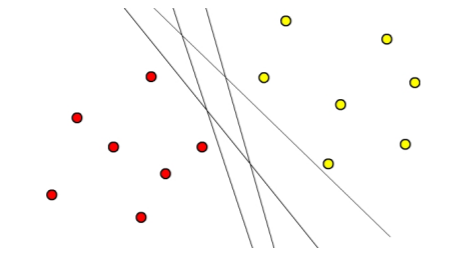
\includegraphics{abbildungen/trennungen.PNG}
	\end{center}
	\caption{Die Abbildung zeigt verschiedene trennende Ebenen für die gelben und roten Datenvektoren.}
	\label{pic-sep-hyp}
\end{figure}

Die Abbildung \ref{pic-sep-hyp} illustriert ein Klassifizierungsproblem bestehend aus roten und gelben Datenvektoren, sowie hierfür zulässige lineare Klassifikatoren im Sinne von (\ref{equ-H}). Das empirische Risiko liefert uns kein Indiz für einen möglichst generalisierenden Klassifikator. Zu erkennen sind jedoch Ebenen mit größeren und kleineren Abständen zu den roten oder gelben Datenvektoren. Im nächsten Unterkapitel werden wir diese Tatsache für die Konstruktion der SVM nutzen. \\

Der nächste Satz \ref{satz-svm-ls} zeigt uns, dass der Abstand der Hyperebenen aus $\mathbb{H}$ sogar beliebig klein zu den Trainingsvektoren beider Klassen werden kann. 
\begin{satz}
	\label{satz-svm-ls}
	Sei $\varepsilon > 0$. Dann existieren ein linearer Klassifikator $h_{(w,b)} \in \mathbb{H}$, sowie $i = 1,...,l,\ j = 1,...,l$ mit $y^i \neq y^j$, sodass $d(E_{(w,b)},x^i) < \varepsilon$ und $d(E_{(w,b)},x^j) < \varepsilon$ gelten.
\end{satz}
\begin{proof}
	Sei 
	\begin{equation}
	\begin{aligned} \label{min-prog-h}
		& \smash{\min_{\substack{(w,b) \\ ||w||=1 }} \; 
				d(E_{(w,b)},x^i) + d(E_{(w,b)},x^j)
		} \qquad \text{u.d.N.} 
		\qquad & y^k(w^tx^k+b) \geq 0 \\
			   && k = 1,...,l
	\end{aligned}
	\end{equation}
	ein Minimierungsproblem mit $y^i=1$ und $y^j=-1$ für $0 \leq i \le j \leq n$. Die Zielfunktion aus (\ref{min-prog-h}) lässt sich weiter zu 
	\[
		 d(E_{(w,b)},x^i) +d(E_{(w,b)},x^j) = y^i(w^t x^i+b) + y^j(w^t x^j +b) = w^t(x^i-x^j)
	\]
	vereinfachen. 
	Die Bedingung $||w||=1$ schließt $(w,b)=0$ als triviale Lösung von (\ref{min-prog-h}) aus. Aus der Separierbarkeit der Trainingsvektoren folgt, dass die zulässige Menge nicht leer ist. Weiter ist die zulässige Menge abgeschlossen. Die Beschränktheit kann man sich wie folgt klar machen: 
	
	Definiere 
	\begin{equation}\label{equ:bounded-set}
	M' := \max_{||w|| = 1}{\max_{1 \leq i \leq l}{y^i \langle w, x^i \rangle}}.
	\end{equation}
	Sei weiter $(w,b)$ für das Problem (\ref{min-prog-h}) zulässig. Wir wollen zeigen dass dann $|b|<M'$ gelten muss.
	Angenommen $b > M'$. Dann folgt mit (\ref{equ:bounded-set}) (und $y^j=-1$) die strikte Ungleichung 
	$$
	y^j(w^t x^i + b) = y^j w^t x^i - b < y^j w^t x^i  - M' \leq 0.
	$$
	Im Widerspruch zur Zulässigkeit von $(w,b)$. Die Annahme $b < M'$ führt zu einem analogen Widerspruch, sodass wir $|b| \leq M'$ fordern können. 
	Damit ist die zulässige Menge abgeschlossen und beschränkt,	nach dem Satz von Heine-Borel (vgl. \cite{ae-ana1}) also kompakt. Da außerdem die Zielfunktion stetig ist, sichert uns der Satz vom Minimum und Maximum  (vgl. \cite{ae-ana1}) die Existenz einer Lösung $(w_{i,j}^*,b_{i,j}^*)$ zum entsprechenden Minimum  $M_{(i,j)}$. 
	Da der Abstand stets nicht negativ ist, folgt $M_{(i,j)} \geq 0$. 
	
	Wir dürfen nach eventueller Umbenennung annehmen, dass $(i,j)$ so gewählt ist, dass die Gleichung 
	$$
	(i,j) = \argmin_{1\leq q,r \leq l} \; \{ M_{(q,r)} \mid (y^q,y^r)=(1,-1) \}
	$$ 
	erfüllt ist, wobei $M_{(q,r)}$ die entsprechenden Lösungen von (\ref{min-prog-h}) für $(q,r)$ sind. \\
	
	Seien nun $M := M_{(i,j)}$, sowie  $(w^*,b^*) := (w_{i,j}^*,b_{i,j}^*)$. Können wir zeigen, dass $M=0$ gilt, ist der Satz bewiesen.
	Um dies zu sehen sei $M=0$ und $(v,p)$ eine separierende Hyperebene der Trainingsdaten. Dann induziert für beliebiges $\beta > 0$ der Vektor $e(\beta) := (w^*,b)+ \beta (v,p)$ einen linearen Klassifikator, also ist $h_{e(\beta)} \in \mathbb{H}$. Jetzt folgt mit
	$$
	\begin{aligned}
	d(E_{e(\beta)},x^{i/j}) &= ((w^*)^t+\beta v^t) x^{i/j} + (b^*+\beta p) = (w^*)^t x^{i/j} + b^* + \beta (v^t x^{i/j} + p) = \\
	&= 0 + \beta (v^t x^{i/j} + p) \xrightarrow{\beta \rightarrow 0} 0
	\end{aligned}
	$$ 
	die Behauptung. \\
	
	Angenommen $M \neq 0$. Da dann $M>0$ gelten muss, ist $d(E_{(w^*,b^*)},x^i) > 0$ oder $d(E_{(w^*,b^*)},x^j) > 0$. \\
	
	Wir nehmen zunächst an, dass der Abstand der Ebene zu einem Datenvektor $0$ ist. O.b.d.A. sei $d(E_{(w^*,b^*)},x^i) = 0$. Den anderen Fall behandeln wir analog. Da dann wegen der Wahl von $(i,j)$
	$$
	d(E_{(w^*,b^*)},x^k) \geq d(E_{(w^*,b^*)},x^j) > 0
	$$ 
	für alle $k$ mit $y^k = -1$ gilt, existiert ein $\bar{b}>0$, dass mit $\bar{e} := (w^*, b^*+ \bar{b})$ der Abstand  $d(E_{\bar{e}}, x^k) > 0$ für alle $1 \leq k \leq n$ ist. Insbesondere ist $\bar{e}$ zulässig für (\ref{min-prog-h}). Weiter ist 
	$$
	d(E_{\bar{e}},x^i) + d(E_{\bar{e}},x^j) 
	 = (w^*)^t(x^i-x^j) 
     = d(E_{(w^*,b^*)},x^i) +d(E_{(w^*,b^*)},x^j),
	$$
	wobei die zweite Gleichheit aus  $y^i+y^j=0$ folgt. 
	Damit wäre $\bar{e}$ eine weitere Lösung des Problems (\ref{min-prog-h}) mit $M > 0$. \\
	
	Es reicht also den Fall $M>0,\ d(E_{(w^*,b^*)},x^i) > 0$ sowie $d(E_{(w^*,b^*)},x^j) > 0$ zu widerlegen. Wir wollen dies mit einem Widerspruch erreichen. Da also in diesem Fall keine der Nebenbedingungen aktiv ist, haben wir die Freiheit die linearen Restriktionen in einer hinreichend kleinen Umgebung von $w^*$ zu ignorieren. Wir suchen jetzt ein $\bar{w}$, sodass
	$$
		\begin{aligned}
		\bar{w}^t(x^i-x^j) &< (w^*)^t(x^i-x^j) \\
		     ||\bar{w}|| &= 1 \\
		 ||\bar{w}-w^*|| &< \delta
		\end{aligned}
	$$
	für ein beliebig klein gewähltes $\delta > 0$ gilt. Transformieren wir das Koordinatensystem über eine (isometrische) Drehung so um, dass $(x^i-x^j)=\eta e_n$ für ein positives $\eta$ gilt, erkennen wir, dass die n-te Komponente $w^*_n$ von $w^*$ wegen
	$$
	\eta w^*_n = (w^*)^t (x^i-x^j) = d(E_{(w^*,b^*)},x^i) + d(E_{(w^*,b^*)},x^j) = M > 0
	$$ 
	positiv sein muss. Wir sind also in der Situation, dass wir auf der Nordhalbkugel von $S^{n-1} := \{x \in \mathbb{R}^n \mid ||x|| = 1 \}$ nach einem $\bar{w}$ suchen, sodass $0 \leq \bar{w}_n < w_n^*$ gilt. Es ist ersichtlich, dass hierfür eine stetige Kurve $\gamma : [0,t_0] \rightarrow S^{n-1}$ mit $\gamma(0) = w^*$ und $ \gamma(t) < (w^*)^t(x^i-x^j)$ für $t \in (0, t_0]$ existiert. Wegen der Stetigkeit von $\gamma$ finden wir schließlich ein $t_1$, sodass mit $\bar{w} := \gamma(t_1)$ der Punkt $(\bar{w},b^*)$ zulässig für ($\ref{min-prog-h}$) ist. Nach obiger Argumentation wäre dann aber $0 \leq \bar{w}^t(x^i-x^j) < (w^*)^t(x^i-x^j) = M$, was nach Konstruktion von $M$ nicht möglich ist. Also muss $M=0$ gewesen sein.
	
\end{proof} 